\chapter{Background Theory}

% \newenvironment{conditions}
%   {\par\vspace{\abovedisplayskip}\noindent\begin{tabular}{>{$}l<{$} @{${}={}$} l}}
%   {\end{tabular}\par\vspace{\belowdisplayskip}}
  
\newenvironment{conditions}[1][where:]
  {#1 \begin{tabular}[t]{>{$}l<{$} @{${}={}$} l}}
  {\end{tabular}\\[\belowdisplayskip]}

\label{ch:background}

\section{Concepts of Causality}

Current supervised Machine Learning techniques are designed to exploit possible relationships/correlations between features and labels in order to produce reliable estimates. Use of this kind of technologies in ambit such as Medicine, Finance and Law are now raising increasing concerns due to the lack of ability in such systems to correctly identify causal relationships and provide explanations about their decisions. One possible solution in order to overcome these type of problems if by taking into account causal relationships.

Causality arises naturally in our daily life every-time we ask ourselves any type of interventional or retrospective question (eg. What if I take this action? What if I would have acted differently?).

As shown in Figure \ref{pyr}, Causal Reasoning can be divided in three different hierarchical levels (Association, Intervention, Counterfactuals). At each level, different types of questions can be answered and in order to answer questions at the top levels (eg. Counterfactuals) are necessary as basis knowledge from the lower levels \cite{tools}. In fact, in order to be able to able to answer retrospective questions, we would expect to first be able to respond to intervention and association type of questions.

\begin{figure}[ht!]%
    \centering
    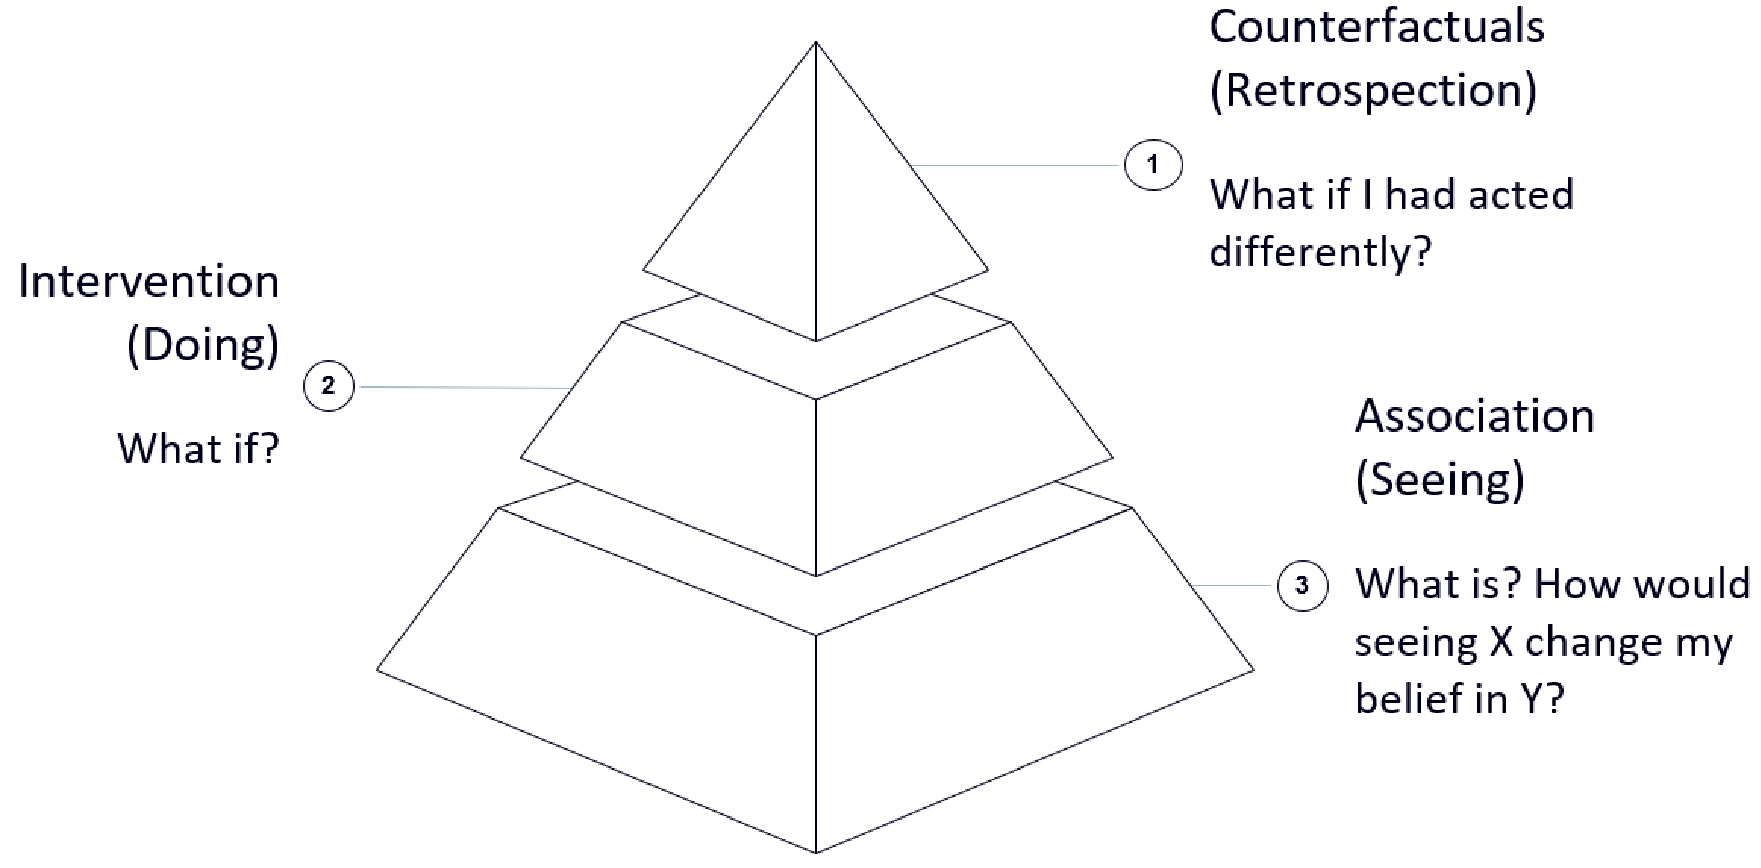
\includegraphics[width=0.8\linewidth]{latex/images/pyramid.pdf}
    % 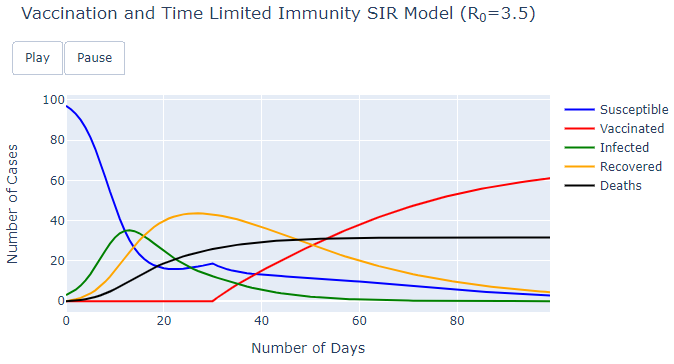
\includegraphics[width=13cm]{latex/images/vacc.PNG}%
    \vspace{-0.2cm}
    \caption{Causality Hierarchy}
    \label{pyr}
\end{figure}
\vspace{-0.5cm}

Currently, Machine Learning models are only able to answer the probabilistic type of questions related to the Association level.
Thanks to the rising interest in this topic, a mathematical framework able to represent causal relationships has been constructed (Structural Causal Models (SCM) \cite{tools}). Using this type of framework, causal expressions can then be formulated and used in conjunction with data in order to make predictions.

This type of framework, can then be divided into two main parts: causal diagrams and a symbolic language. The causal diagrams can be used in order to summarise our knowledge about the topic, while the symbolic language can be used to express what we are aiming to find out.

As an example, let us consider the diagram shown in Figure \ref{dig_ex}. Using this type of representation, the arrow directions indicate how the different variables effects each other.

In this example, a survey is carried out between individuals of age 3-20 in order to find out if there is any correlation between height and Individuals Intelligence Quotient (I.Q.) Scores. Although the study might result in a positive correlation between the two different variables, a more in depth analysis might instead show how height does not directly cause higher I.Q. Scores but these two variables are instead dependent on a third hidden variable (Confounder). In fact, as children grow up, over time both their I.Q. Scores and height tends to increase thanks to their improved education and greater age.  

\begin{figure}[ht!]%
    \centering
    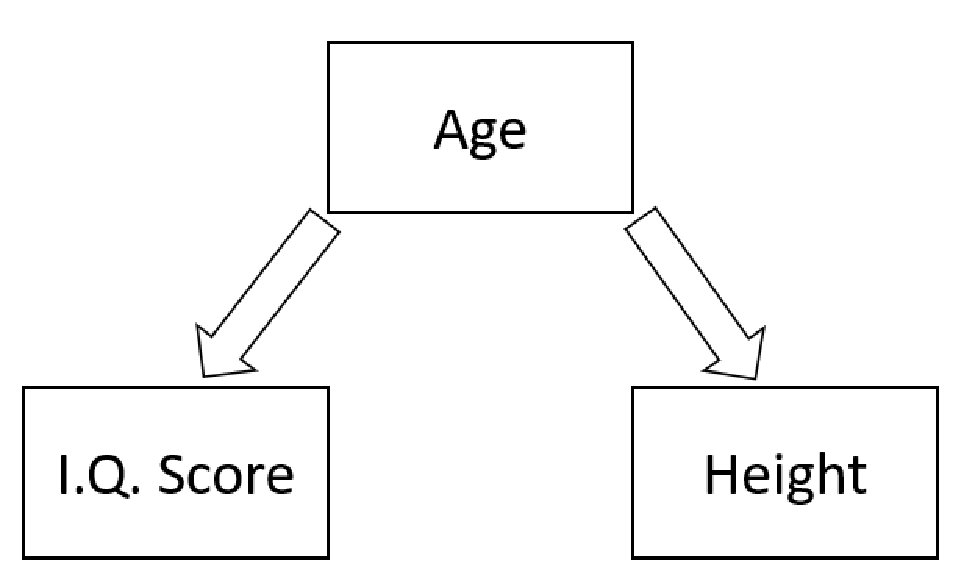
\includegraphics[width=0.4\linewidth]{latex/images/caus_d.pdf}
    \vspace{-0.2cm}
    \caption{Causality Diagram}
    \label{dig_ex}
\end{figure}
\vspace{-0.5cm}

In case we want to query additional information from what we currently have available \footnote{So that to move from the association to the intervention level in the causality hierarchy.}, we can then make use of the symbolic language in order to advance questions such as: What is the probability (P) that a student will get an higher I.Q. score (S) if he studies an additional amount of time (T)? This question could then be formulated in a symbolic form such as $P(S|do(T))$  \footnote{Although, Do-Calculus notation might look similar to the one of conditional probability, the two have two different meanings.}. When formulating these type of questions, we are then implying that we are not anymore passively observing possible results but instead actively intervening in order to find out about possible consequences. This type of approach is known as an Interventional Study and is in contrast with the traditional Observational Study.

Finally, in order to create a full Causal Inference Engine, an architecture like in Figure \ref{engine}, might be necessary \cite{why}. Following this type of approach, three inputs are needed and three outputs are produced. As our three inputs, are given any assumption made about the model (\textbf{Assumptions}), any questions we are trying to answer (\textbf{Queries}) and any data which can be used in order to fuel our engine (\textbf{Data}). The model, will then output as Boolean value if is able or not to answer the given queries, and if so, it would provide as second output a mathematical formula which can be used in order to answer the queries. Finally, a numerical prediction specific to the given input data is provided (this might contain some form of uncertainty in the estimation given the amount of data provided and the assumption made).  

\begin{figure}[ht!]%
    \centering
    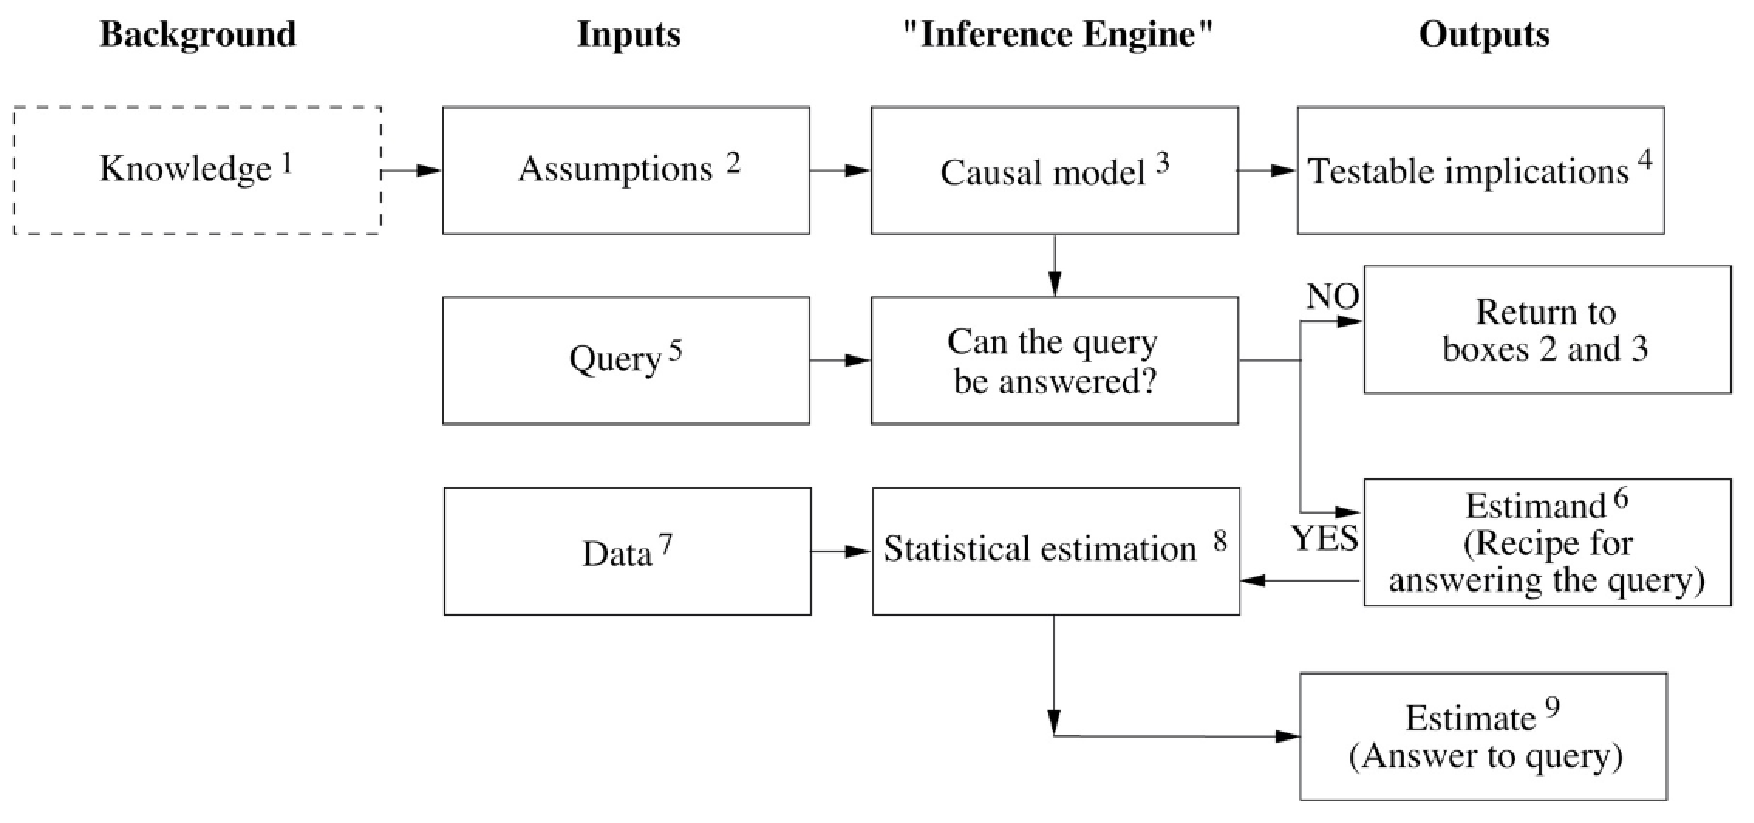
\includegraphics[width=0.8\linewidth]{latex/images/engine.pdf}
    \vspace{-0.2cm}
    \caption{Causal Inference Engine (Image reproduced from: \cite{why})}
    \label{engine}
\end{figure}
\vspace{-0.5cm}

Using this type of paradigm, can ultimately make our model much more flexible than contemporary deep learning models (in fact, our model is now much less dependent on the data and more focused about intrinsic relationships and connections).

\section{Linear and Non-Linear Causality}
\vspace{-0.1cm}
Causality, can be divided into two main types: linear and non-linear (Figure \ref{wow}) \cite{system}: 
\vspace{-1.3cm}
\begin{itemize}
    \setlength\itemsep{-0.5em}
    \item In linear causality, connections between the variables can be in a single direction and every effect can be originated by a limited number of causes. Causes always linearly precedes effects (time precedence).
    \item In non linear causality, connections between variables can be bi-directional and effects can possibly be originated by an unlimited number of causes.
\end{itemize}
\vspace{-0.4cm}
Linear causation systems are characterised by proportional relationships between cause and effects variables (e.g. Deterministic Systems). Instead, in non-linear causation systems disproportionate effects can take place (e.g. Non-deterministic Systems). For example, small changes in input conditions would then result in different consequences (e.g. "Butterfly Effect").
\vspace{-0.1cm}
\begin{figure}[ht!]%
    \centering
    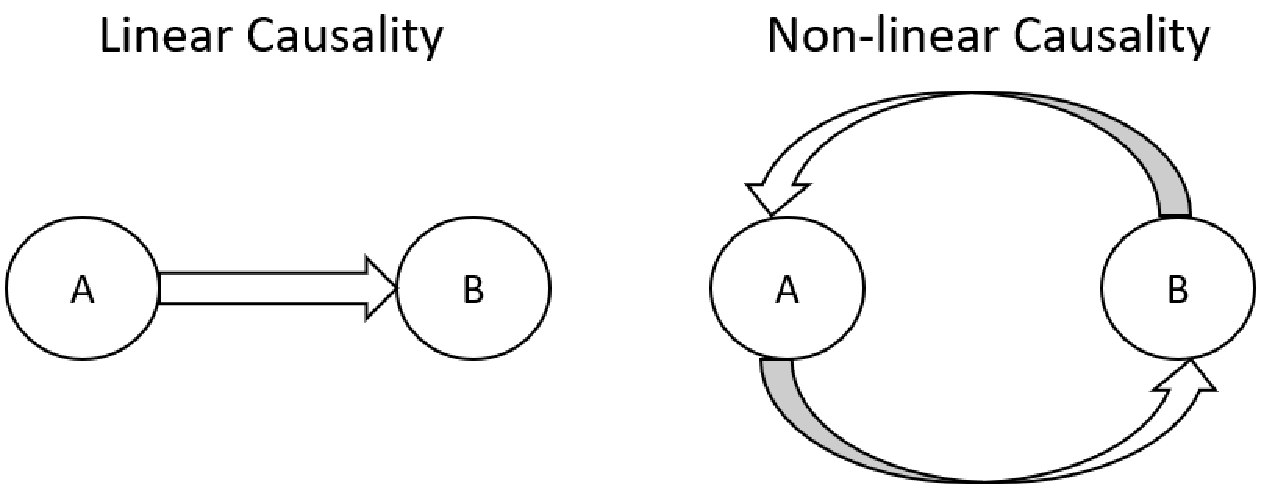
\includegraphics[width=0.7\linewidth]{latex/images/linear.pdf}
    % 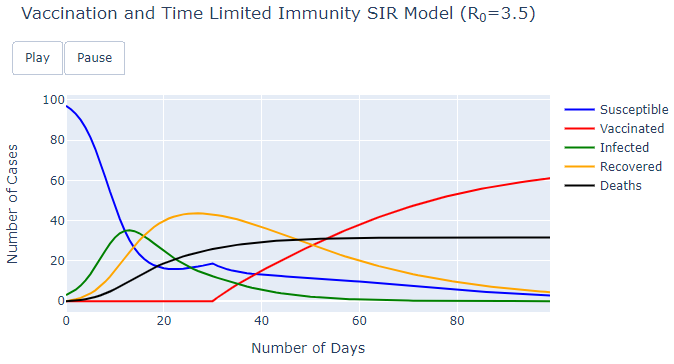
\includegraphics[width=13cm]{latex/images/vacc.PNG}%
    \vspace{-0.2cm}
    \caption{Linear vs Non-Linear Causality}
    \label{wow}
\end{figure}
\vspace{-0.5cm}

From an external point of view, each causal systems can then be characterised as a composition of events, which although might be regulated by a series of hidden trends and rules. Being able to correctly identify how these different constituent forces are interconnected each other (grasping any reciprocal causal mechanism), would then allow us to make any system much more predictable. 

The causal analysis of any dynamical system, could then be summarised by the following workflow (Figure \ref{wow2}). 

\begin{figure}[ht!]%
    \centering
    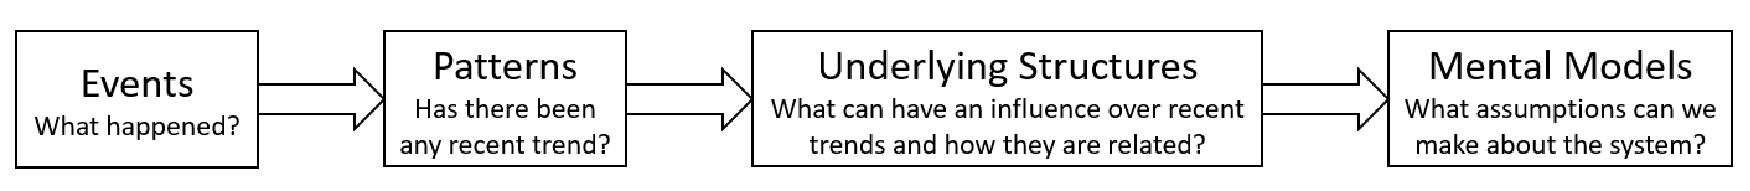
\includegraphics[width=1\linewidth]{latex/images/discover.pdf}
    % 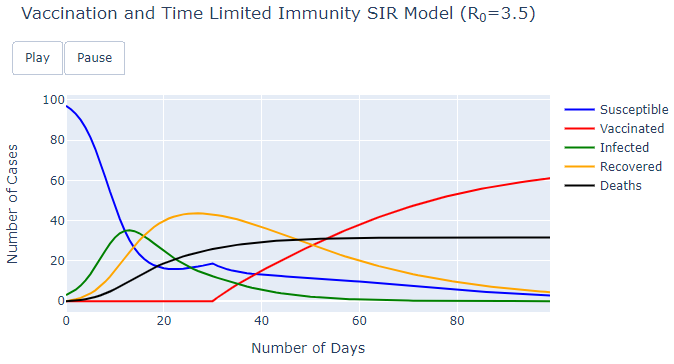
\includegraphics[width=13cm]{latex/images/vacc.PNG}%
    \vspace{-0.6cm}
    \caption{Dynamical Systems Analysis (Adapted from \cite{system})}
    \label{wow2}
\end{figure}
\vspace{-0.5cm}

\section{Case Study: Recommendation Systems}

One of the main weakness of most Machine Learning models is the assumption that the data fed in is independent and identically distributed (IID). When this assumption holds, convergence to the lowest possible loss is achievable but when this constrain is violated the model might perform poorly even when attempting simple tasks (eg. poisoning attacks) \cite{six}.
As an example, let us consider an e-commerce recommendation system. Nowadays systems, are able to offer recommendations mainly based on products correlated to the ones we are planning to buy, although this cannot always lead to accurate estimates. For instance, we might have recently bought a new phone and we are now looking for a phone case. While browsing for phone cases, although our recommendation system might try to suggest us other items such as phones (just because they are correlated) instead of more cause-effect related items like screen protectors.

% \section{Autism Spectrum Disorders (ASD)}

% Nowadays, there does not exist a recognised medical test for autism diagnostic. Cases are examined individually by doctors for classification. Online screening tools such as Q-Chat are currently available to help parents understand if their child is affected or not by autism \cite{screening}. Uses of Machine Learning (to analyse patients EEG readings) and Computer Vision \footnote{to detect, from video recording, behavioural and communication impairments} might provide a useful solution to this problem. 

% Each LSTM module can be considered to be formed by three gates: input ($i_{t}$) , forget ($f_{t}$) and output gate ($o_{t}$). The input gate decides if a piece of information is important enough or not to be remembered (Equation 2.1). The forget gate (Equation 2.2) decides if a piece of information stored is still relevant or not (and therefore has to be deleted). The output gate determines if a particular information has to have or not a weight in the current time step (Equation 2.3).
% \useshortskip
% \begin{align}
% \ i_{t} = \sigma(w_{i}[h_{t-1},X_{t}] + b_{i}) \\
% \ f_{t} = \sigma(w_{f}[h_{t-1},X_{t}] + b_{f}) \\
% \ o_{t} = \sigma(w_{o}[h_{t-1},X_{t}] + b_{o})
% \label{eq:3}
% \end{align}
% \useshortskip
% \begin{conditions}
%  w_{x}  &  neuron gate weight \\
%  h_{t-1}     &  LSTM previous step output \\
%  X_{t}     &  LSTM current input \\   
%  b_{x}      &  gates biases \\
% \end{conditions}
% \useshortskip
% The Sigmoid function ($\sigma$, Equation 2.4) is used to squish the output between any value from zero (making the gate block everything) to one (making the gate pass through everything). A neuron gate weight ($w_{x}$) represents the strength of the connection, while the bias ($b_{x}$) is used shift the activation function to fit best the data.

% \useshortskip
% \begin{align}
% \ \sigma(x) = \frac{1}{1 + e^{-x}}
% \label{eq:3}
% \end{align}
% \useshortskip

% In mathematical terms, convolution ($\circledast$) is an operation between two functions to create a third one, which represents to what extent a function can be modified by another (Equation 2.5).
% \begin{align}
% \ (f \circledast g)' = \int_{\infty}^{\infty} f(\tau)g'(t-\tau)d\tau
% \label{eq:3}
% \end{align}
% \useshortskip

% {
% \begin{table}[h!]
% \centering
% \begin{tabular}{l|l|c|c|c}
% \multicolumn{2}{c}{}&\multicolumn{2}{c}{Model Predictions}&\\
% \cline{3-4}
% \multicolumn{2}{c|}{}&Negative (0)&Positive (1)&\multicolumn{1}{c}{Total}\\
% \cline{2-4}
% \multirow{}{}{True Outputs}& Negative (0) & $TN$ & $FP$ & $TN+FP$\\
% \cline{2-4}
% & Positive (1) & $FN$ & $TP$ & $FN+TP$\\
% \cline{2-4}
% \multicolumn{1}{c}{} & \multicolumn{1}{c}{Total} & \multicolumn{1}{c}{$TN+FN$} & \multicolumn{    1}{c}{$FP+TP$} & \multicolumn{1}{c}{$N$}\\
% \end{tabular}
% \caption{Confusion Matrix}
% \label{table:1}
% \end{table}
% }

% Using the Confusion Matrix, the model Accuracy can be also calculated as:
% \begin{align}
% \ Accuracy (ACC) = \dfrac{TP + TN}{TP + TN + FP + FN}\times100\% 
% \end{align}

% From the Confusion Matrix it is then possible to calculate a model Sensitivity and Specificity. In a medical context, sensitivity quantifies the model's ability to determine patients effected by a certain medical condition. Specificity instead measures the model ability to correctly identify patients not effected by this condition.

% \begin{align}
% \ Sensitivity (TPR) = \dfrac{TP}{TP + FN}\times100\% \label{eq:1} \\
% \ Specificity (TNR)  = \dfrac{TN}{TN + FP}\times100\%
% \end{align}

% The AUC (Area Under The Curve) - ROC (Receiver Operating Characteristics) curve evaluates a model's ability to correctly discriminate between the different classes using different thresholds. 

% Plotting the False Positive Rate (Specificity) against the  True Positive Rate (1 - Sensitivity), the ROC Curve can be calculated (Figure 2.10).